\chapter{Problem modeling}\label{chap:formulation}
% comit 21-11-2017
\minitoc

%----------- newPlane  ----------
%%%%%%%%%%%%%%%%%%%%%%%%%%%%%%%%%
%\section { The map}
%	\subsection{...}
%	\subsection{...}
%\section{Camera definition}
%
%\section{Cost Function}
%	\subsection{Constraint}
%	


%%%%%%%%%%%%%%%%%%%%%%%%%%%%%%%%%

%The following chapter is focused on the problem formulation for cameras positioning.\\
%Obviously formulation proposed in not the only one and some other have been proposed in the literature, mostly depending then the objectives. \\

%The problem formulation has to translate the objective with all this problematic into a simple formulation usable for different optimization algorithms. 
The following chapter is dedicated to the in details formulation of the problem of cameras positioning . 
The objective here is to find the position for a camera set or waypoints. The position of this set of waypoints has to be optimized in order to cover most of the area. The area that has to be covered may be vast and composed of complex zones.
A good formulation is essential to design an efficient cost function. The cost function is used to quantify the quality of the solutions. It is a crucial element for the optimization processes.\\
This chapter present a formal definition of the problem based on the literature as well as our proposed formulation. 
The formulation proposed is adapted to optimize the problem of cameras or waypoints positioning depending on many constraints such as  a complex and vast map or  cameras mounted on UAVs.
%The formulation proposed is adapted to optimize the problems with evolutionary algorithm to have an efficient cameras position for maximizing the coverage, depending then many constraints as for example using a camera mounted on UAV.

%\section{Coverage estimation }


The following sections are focused on the estimation of the area coverage  depending on the camera parameters.\\

%What should be control by the video surveillance? \\
%One aim of the video surveillance is to detect some anomaly in the area for that the number of black hole need to be reduce. A black hole is zone not cover by the system of video surveillance. Estimate the part cover by the system of video surveillance is primordial to limit the size and the number of black hole. 
%To know if the area is cover by a minimum of one vision sensor, different techniques can be used.
%Indeed the coverage estimation is essential element to optimise the position of a network of cameras. But before to find the position some assumption should be done to describe our problems and explain the methodology to calculate the coverage rate of an area.
%The main purpose of our work is to estimate the position for the vision sensors network into a given area.\\
%Where the main goal is to manage the positioning of the fix number of cameras in order to maximize the visual coverage. 
%Indeed before to find the position some assumption should be done to describe our problems.\\ 


%To have an efficient optimization, the estimation of the answer are essential. Here the first element to evaluate the answer is the area coverage by a set of cameras mounted on a UAV. \\


%The problem needs to be formalized in order to clearly identify the complexity of the cameras positioning. 

To estimate efficiently the area covered by a given camera set, some points needs to be clearly defined.
First of all the area itself. The question of "How could we represent the area?" is  primordial. The camera definition  with the question of  "How could we estimate the camera projection?" is also an important part of the problem design.  The third part to take care is the constraints which must be added to the systems.
%\begin{itemize}
%\item The area himself. How to represent the area. 
%\item The camera definition. How to estimate the cameras projection.
%\item The constraints added to the systems (constraints and secondary objectives). \\
%\end{itemize} 
  These three parts are discussed in the following sections. The area definition is discussed in the section \ref{sec:Grid} which focus on the grid design. The camera definition is discussed in the section \ref{sec:CamerasCoverage} and the third part about the constraints is addressed in the section \ref{sec:constraint}.\\
Finally, when the problem is clearly defined, all the different elements are integrated to obtain an efficient cost function operable for the optimization process in \ref{sec:costFun}.

   
%;;;;;;;;;;;;;;;;;;;;;;;;;;;;;;;;;; to do ;;;;;;;;;;;;;;;;;;
%
%The term coverage denote the area visible by at least one camera. Also the area to cover represent all the parts of the area which must be control by at least one camera. \\
%
%The area definition is primordial to the coverage estimation the folowing parts is focus on it . 
%The area covered by the set of the cameras will be the based of the cost function. In the second time the cost function will be updated by adding the constraints due to the systems.\\
% 
%Therefore the problem is formulated as:
%\begin{itemize}
%\item [-] Maximization of the coverage with a fix number of cameras.
%\item [-] Minimization of the constraints.\\( as examples the complex shape of the area, the bound of the area, the altitude of the cameras,...)
%\end{itemize}

%%%%%%%%%%%a
%Due to this formulation, composed by the maximisation and minimization, the solution  have to evolve to a best  possible answer based on the cost function. Depending then the formulation of the area and the design of the cost function the ability to optimize a solution is greatly affected. 
%The positions of the cameras have to limit the number and the size of black
%holes to be exploitable. The black holes are the area not covered by the camera
%views. To do so a precise estimated of the part covered by the system of camera views is elemental.\\
%
%
%In order to estimate the coverage properly the area must be discretized. Once the area discritezed it became easier to verifies if each point of the area are coverer by at least one camera of the network.
%%%%%%%%%%%%%%a
%The coverage problem must be modelled properly. The different method to design the problem will affect the solution and the applicable resolve method. The following part will talk about it \\
%The coverage problem must be modelled properly. The different method to design the problem will affect the solution and the applicable resolve method. \\
%The first part is to estimate properly the coverage of the area. To do so many method have been developed most of them are based on the occupation grid $G$ of the area. \begin{equation}
%G=\begin{bmatrix}
% g_1 ...g_i ... g_m
%\end{bmatrix}  , m\in \mathbb{N}
%\end{equation}
%Where $m$ is the number of points in the grid.
%The occupation grid is mostly placed on the floor of the area to cover. At minima each point $g_i$ of the grid $G$ should be cover by the vision sensors. Consequently a list of points is created to listed the covered part of $G$ which are noted as $Pc$.
%\begin{equation}\label{eq:Pci}
%g_i \in Pc \mbox{ IFF } g_i \mbox{ is coverd. }
%\end{equation}
%
%The modelization of the grid is an important element and different solution has been proposed during the time with different advantage depending then the situation.\\

\section{The map}\label{sec:Grid}


%/!$\backslash$ \textbf{ ajouter une partie dedier  a [181*] qui propose une solution pour ajusté la densité en fonction  de la necesité de présision  (contour plus dense ) }

The first part is equivalent to the estimation of the area that needs to be covered. Following this direction, many methods have been developed and most of them are based on an occupation grid $G$ of the area. The occupation grid is a discretization of the area with numerous points.
\begin{equation}\label{eq:Grid}
	G=\begin{bmatrix}
	 	g_1 ...g_i ... g_m
	\end{bmatrix}  , m\in \mathbb{N}
\end{equation}
Where $m$ is equal to the number of points in the grid.
The occupation grid is placed on the area to cover. Each point $g_i$ of the grid $G$ should be covered by a camera. In the Figure \ref{fig:cam_projOnGrid} the grid $G$ and the points $g_i$ are represented, as well as one camera and this associate projection on to the grid.
 Consequently some parts of the grid is covered (red dot in the Figure \ref{fig:cam_projOnGrid}). 
% Consequently the list of points is set up to enumerate the covered part of $G$ which are noted as $Pc$. 
%\begin{equation}\label{eq:Pci}
%g_i \in Pc \mbox{ IFF } g_i \mbox{ is coverd. }
%\end{equation}
\begin{equation}\label{eq:B}
\forall g_i \in G, B(g_i)= \begin{cases} 1, & \mbox{if } g_i \mbox{ is covered by at least one camera }\\ 0, & \mbox{otherwise}   \end{cases}
\end{equation}
$B$ is the set of grid points which associate the value  "1"  if covered by at least one of the camera. The size of $B$ is relative to the size of $G$.
\begin{figure*}[t!]
		\centering
		\minipage{0.85\textwidth}
  		\includegraphics[width=\linewidth]{img/CamProjectOnGrid2.png}
  
 	 	\endminipage\hfill\caption{Camera projection onto a grid. The grid $G$ is placed on the floor to discretize the area covered with numerous grid points $g_i$. The point covered by the camera, belonging to $B()$ are highlighted in red.}\label{fig:cam_projOnGrid}
\end{figure*}
\\ The design of the grid is an important element of the problem formulation. Many solutions were proposed, with different advantages depending on the situation (constraints and objectives).\\

\subsection{Designing a grid map} \label{sec:GridMap}%Related work for the grid design

The following section is focused on the different grids design proposed in the literature. The usage of grid to describe the area that must be covered is common and several designs have been invented and used depending on the constraints and objectives.  


\subsubsection{Sampling frequency} %Sampling frequency.\\
The grid map is used to discretize the application area. The discretization of the area may vary and the area can get a high or low level of discretization. The level of sampling frequency has a bearing both on the problem formulation and on the optimization process.

\paragraph*{High sampling frequency}
%The high level of discretization or high sampling frequency has some advantage and disadvantage.\\ 
The high level of discretization or the high sampling frequency of an area is characterized by a big amount of point $g_i$ to describe an area. The big amount stands for having an important density of point $g_i$ and consequently a high value of $m$. 

%\begin{equation}
%	G=\begin{bmatrix}
% 		g_1 ...g_i ... g_m
%	\end{bmatrix}  , m\in \mathbb{N}
%\end{equation}
%
%Where m is the number of point into the grid.
% \subparagraph{Advantage of the  high sampling frequency.}
%////////////high sampling advantage////
The main advantage of this approach lies in having a better estimation of the coverage. The more the area is finely discretized, the more the estimation of the coverage will be sharp. In \citep{171*horster2006}, an example of high frequency sampling is given in order to have sharp estimation of the area. \\
The high sampling frequency allows the cameras position to be much more accurate and requires smaller adjustments.
%////////////high sampling disadvantage////\\
\\On the other side, a too high sampling frequency leads to high computation time. Rather to refine the solution, a too high level of discretization of the area will make the optimization longer and more complex. Indeed, to control the coverage, it is necessary to control if each point of the grid is covered by a camera.  
%\begin{equation} 
%	\sum^m \sum^n \mbox{test of coverage}
%\end{equation}
%Where $m$ is the number of points in the grid and $n$ the number of camera. 
%That mean the number of test to estimate the coverage of each point of the grid, for a given set of cameras is $m\times n$. Where $m$ is the number of points in the grid and $n$ the number of camera. \\
 The more the size of the grid, the more unity test of coverage (see in Section \ref{sec:CamerasCoverage}) are necessary, and it impacts each step of the optimization process. Consequently the size of the grid will greatly affect the computation time.  \\
Also the high sampling frequency will affect the positioning of the cameras pose. In fact, higher is the sampling frequency of the area, freer the pose estimation of  each camera will be.


%////////////////////////////////////

%In fact the quality of the coverage estimation affect the positioning optimization. %A bad estimation of the area coverage due to the bad level of discretization will impact the quality of the answer and the precision of the cameras position by returned a approximate coverage rate. 
\paragraph*{Low sampling frequency}
%///////////////////advantage of the low sampling///////
At the opposite, a lower sampling frequency can be a good solution to upgrade the convergence speed of the optimization process as this behavior has been presented in \cite{8*zhou2011}. In Zhou et al \cite{8*zhou2011}, a small value of $m$ is chosen to have a real time solution for small areas with just few cameras (up to  20). 
%////////////low sampling disadvantage////
On the other side, the low sampling frequency may generate a bad estimation of the area covered due to the too low density of points in the grid. The low density of points may give an approximate view of the covered area and some uncovered areas (black hole) can appear between the points of the grid. These uncovered areas can be too small to be detected due to the low density of points. In this case, the optimization cannot take into account the uncovered area sand the solution given after an optimization will be, in a real environment, of bad aspect. Concretely, the difference between the coverage estimation of the discrete area and the  coverage estimation in continuous time must be high.    \\



%////////////////////sumup//////////

% tableau auto généré   bug 
%\begin{table}[]
%\centering
%\caption{My caption}
%\label{my-label}
%\begin{tabular}{l|l|l|}
%\cline{2-3}
%\textbf{} & \textbf{Avantage} & \textbf{Disadvantage} \\ \hline
%\rowcolor[HTML]{FFFFFF} 
%\multicolumn{1}{|l|}{\cellcolor[HTML]{FFFFFF}} & Best estimation of the area to cover & \cellcolor[HTML]{FFFFFF} \\
%\multicolumn{1}{|l|}{\multirow{-2}{*}{\cellcolor[HTML]{FFFFFF}\textbf{High sampling frequency}}} & Give more precision on the cameras poses & \multirow{-2}{*}{\cellcolor[HTML]{FFFFFF}Time consuming} \\ \hline
%\rowcolor[HTML]{EFEFEF} 
%\multicolumn{1}{|l|}{\cellcolor[HTML]{EFEFEF}\textbf{Low sampling frequency}} & Faster computation & Bad coverage estimation \\ \hline
%\end{tabular}
%\end{table}
\paragraph*{Low or high sampling frequency}
Finally, the too low sampling frequency, instead of gaining computation time, may affect the quality of coverage  estimation. Contrarily, the impact of a too high sampling frequency has consequences, as summarized in the Table \ref{tab:samplingFrequency}. The sampling frequency should be carefully estimated. \\
The density of the grid has to be adjusted depending on the goal and the precision required. One of the solutions proposed in Zhao et al \citep{22*zhao2008} is a progressive refinement by increasing the grid density.
%////////////progressive sampling/////
Zhao et al \citep{22*zhao2008}, despite a low density of points at the beginning,  proposef to increase the number of points slowly to obtain a better density and refined results. Also the increasing points frequency is applied to refine the solution and add more cameras at each step of the optimization leading to avoidance of uncovered area.  \\


%////////////camera pose estimation linked//////////////////////
%!!!!!!!!!!!!!!!!move it somewhere!!!!!!!!!!!!!!!!!!!
\subsubsection{Cameras pose precision}
The sampling frequency  of the grid is often linked to the pose precision of the camera as discussed previously. In some cases, such as in  \citep{83*van2009,150*chakrabarty2002,195*choi2009,87*morsly2012}, the available position of the cameras are strongly linked to the grid map and the sampling frequency.
 %The search space represent the domain to optimize or can be defined by the set of all possible solutions in our case the search space is all the position for all the cameras. 
Increasing the number of points in the grid will also increase proportionally the number of possible positions for each cameras. More the area is finely defined more it is necessary to slightly adjust the cameras positions. Consequently the possible camera positions and the search space are increased to finally allow a more refined solution but also a more complex one.

On the other hand, the camera poses can be limited at some specified areas of the map. In \citep{171*horster2006,22*zhao2008}, the cameras can be placed against the walls. In \cite{22*zhao2008}, every wall  of the boundaries can hold a camera. In \cite{171*horster2006}, the camera can be placed only on specified zone (as shown in the Figure \ref{fig:randomGridRef171}, the green wall shows the available position of the cameras).

The camera poses precision has a similar impact and consequence on the result as the grid map.
A to big  number of possible poses allows an increased precision but greatly increase the complexity, while a too small  number of possible poses helps to converge faster but will lead to lower precision. 
 %151*
 %The too high precision in the position of the camera will increase the complexity and some case where the value of $m$ is too high the optimization process cannot converge or find acceptable solution to the gain of the search space. \\ 
%\\!!!!!!!!!!!!!!!!!!!!!!!!!!!!!!!!!!!!!!!!!!!!!!!!!!!
% 171*  cam position sur les mure  see fig 4.3
%22*   came position on the wall
%151* cam pos wall 
%8*  camera  free position low sampling F
%83*  camera position is a miroring of the grid map
%150*  capteur pose topologique 
%195*  hover robot   218
%215*  hover roboto exploration 
\subsubsection{Distribution}
The distribution of the points over the grid, is an important factor to manage for the design of an occupation grid.% The distribution is how the points of the grid are placed on the area to cover.
 The points distribution can numerous and adapted to different specific case. Mainly two distribution are used. The grid pattern distribution is the more often seen in the literature and in a lesser extent the random distribution. These two distribution  are illustrated in the Figure \figref{fig:GridVsRand}.

%Different distributions can be used, but commonly in the literature the grid pattern distribution and in a lesser extent the random distribution is applied (see Figure \figref{fig:GridVsRand}). 
\begin{mfigures}[!]
{Map representation using random distribution or uniform grid.}{fig:GridVsRand} \centering
\mfigure{width=.4\linewidth}{img/GridVsRand1.png}{Grid with uniform and regular distribution.}{subfig:satimgTorcy}
\hspace{1cm}
\mfigure{width=.4\linewidth}{img/GridVsRand2.png}{Random distribution for represent the map.}{subfig:satimgMaskTorcy}
\end{mfigures}

%\begin{figure}[t!]
%\begin{center}
%\minipage{0.65\textwidth}
%   \includegraphics[width=\linewidth]{img/GridVsRand.png}
%  \caption{ (a)Grid with uniform and regular distribution.\\   
%(b) Random distribution.\\  
%}\label{fig:GridVsRand}
%  \endminipage\hfill
%  \end{center}
%\end{figure}
%%%%% FIGURE  random distribution  form 171*
\begin{figure}[t!]
\begin{center}
\minipage{0.65\textwidth}
   \includegraphics[width=\linewidth]{img/randomGridRef171.png}
  \caption{Example of  map that must be  covered with a randomized area sampling. Illustration from Horster et al \citep{171*horster2006} \\
  (a) Area  to cover.\\ 
  (b) Area with the random points of the grid to cover \\
  (c) Importance weighting of the area (zone of the interest).\\  
  (b) allowed position for cameras position.}\label{fig:randomGridRef171}
  \endminipage\hfill
  \end{center}
\end{figure}

 The random distribution is used to describe the area to cover as  shown in \cite{83*van2009,171*horster2006}. \\
In Hoster et al \citep{171*horster2006}, the points of the grid are randomly distributed to describe the area to cover. The advantage of this article remains the usage of random distribution to manage the density of points in some specific regions of the area. Especially, by increasing the density of points on some specific zones of the area. The increased density allocates more importance to these zones (see Figure \ref{fig:randomGridRef171}).\\
Indeed, higher density will affect the optimization process. The area with more density will be comparatively more profitable to a low density area. In these cases, the zones with high density are covered in priority. This mechanism is even simplified due to the random distribution.

Hengel et al \cite{83*van2009} have tested the random distribution and the uniform grid pattern distribution before conclusing that the grid pattern and the random distribution proposes globally observe the same result when there is no priority zones in the area. Based on this observation, authors (Hengel et al \cite{83*van2009}) decided to use an uniform grid because of its simplicity of implementation.
%///////random distribution   for reduce the uniforme grid //////////
A  hybrid distribution is proposed in  Zhao et al \cite{22*zhao2008}.
%The "random distribution" is less popular but in  a hybrid distribution is proposed. 
The idea is to reduce the number of points in the uniform grid when it has a to high density. To reduce the number of points in the grid, a random selection is applied. This hybrid implementation of an uniform grid with a random selection to decrease the sampling frequency is an example of hybrid distribution.


\subsubsection{Spatial modelling (3D or 2D)}
 The spatial modelling has an important impact on the grid design. After imposing the necessary density and the distribution of the grid, the position of the points $g_i$  in space which composes the grid  has to be discussed.  
%In fact depending on the problem the grid can be modelled differently in order to properly cover the area to control.
  Commonly, the occupation grid is placed on the floor and calculate visibility only in 2D  by computing the  camera projection as in  \citep{164*valente2013,150*chakrabarty2002,8*zhou2011,170*yabuta2008,171*horster2006,22*zhao2008}. But depending on the context, the grid could have interest to describe a 3D space.  
Hengel et al \cite{83*van2009} calculated the visibility according to relevancy: for example, on the upper torso or head of the possible target rather than on the floor. In this case, a 2D grid is proposed inside the 3D space in order to  characterize properly the volume by placing the grid at a specific height.  

In Chrysostomou et al \cite{82*chrysostomou2012} or also in \cite{226*nazarzehi2018}, the grid is formalized in the full volumetric space by numerous “control points” to control the area (illustrated in Figure \ref{fig:3Dgridfrom226}). The points of the grid are uniformly distributed along the axis of $x, y$ and $z$. The grid are formulated in the volumetric space by using an uniform 3D grid distribution.
The uniform grid distribution in a 3D space increases greatly the complexity  due to the important augmentation of control points ($g_i$) and their respective dispersion. Its implementation is unusual due to the increasing difficulty of the optimization process. 
To avoid the increasing complexity, the 3D grid is replaced by a  2D grid in the beginning at a specific height to optimize the coverage. 
 %The formulation proposed shown the complexity even more important to use a 3 dimensional occupation grid. For practical reasons, mostly the inadequacy has computational power due to the increased complexity, the 3D grid is replaced by a 2D grid at a specific height to optimize the coverage. 
%While an occupation grid designed to estimate the volume cover along the $ x, y $ and $ z $ axes of the area already exist. %His implementation is unusual due to the increasing difficulty of the optimization process.  
Nevertheless, some solutions were discussed \citep{141*akbarzadeh2013,83*van2009} to take into account the volume of the area that must be covered which cannot be only limited to an occupation grid along the axes $ x $ and $ y $ as if using a 2D grid.
\begin{figure}[t!]
\begin{center}
\minipage{0.65\textwidth}
   \includegraphics[width=\linewidth]{img/3DgridFrom226.png}
  \caption{3D grid with uniform distribution of the grid points. Illustration from \cite{226*nazarzehi2018} }\label{fig:3Dgridfrom226}
  \endminipage\hfill
  \end{center}
\end{figure}

In  Hengel et al\cite{83*van2009}, the authors were focused on estimating the area to cover inside three floors of a building. To estimate the coverage in the building, the grid was placed at each floor. This solution is efficient in order to limit the number of grid points compared to a full volumetric description of the area. Also, this design allows to keep the three dimensional information by adding a layer at each level of the building (see Figure \figref{fig:gridByLevel83}). 
 %*** from 83 ***
 \begin{mfigures}[!]{Illustration of a grid layer in three floor building from \citep{83*van2009}. In the figure (b) (d) (c) the uniform grid is visible with the black case of the grid representing the area uncovered and the colored case for the covered area.}{fig:gridByLevel83} \centering

\mfigure{width=.4\linewidth}{img/buldingViewfrom83.png}{Building view.}{subfig:r4}
\hspace{1cm}
\mfigure{width=.4\linewidth}{img/Level1from83.png}{1$^{st}$ floor.}{subfig:r1}
\hspace{1cm}
\mfigure{width=.4\linewidth}{img/Level2from83.png}{2$^{nd}$ floor.}{subfig:r2}
\hspace{1cm}
\mfigure{width=.4\linewidth}{img/Level2from83.png}{3$^{rd}$ floor.}{subfig:r3}


\end{mfigures} 

Another way to deal with a volumetric space while not using a greedy 3D grid distribution lie into adaptation of the 2D grid onto the relief. Akbarzadeh et al\citep{141*akbarzadeh2013} proposed a 2D grid adapted to the relief of the area. This article is focused on covering a large outdoor area with an important relief (hills and valleys). To estimate properly the area to cover, a grid was placed following the altitude of the relief as shown in Figure \ref{fig:grilleRef141}. The spatial modeling is traditionally a 2D grid at fixed altitude more or less equal to the floor ground. 
The 2D grid distribution adapted to a 3D environment is the easiest and can be customize for numerous problems which allows the reduction of the number of control points ($g_i$) and thus  the computation time. 

%%% figurir  from 141*
\begin{figure}[t!]
\begin{center}
\minipage{0.65\textwidth}
   \includegraphics[width=\linewidth]{img/grilleRef141.png}
  \caption{Relief grid used to discretize  an area while taking into account the relief. Illustration from \cite{141*akbarzadeh2013} }\label{fig:grilleRef141}
  \endminipage\hfill
  \end{center}
\end{figure}

\subsubsection{Zones of interest} \label{sec:zoneOfInterest}
Among the areas to cover, some zones may have a particular interest to be covered. These zones can be discriminated by the grid design. 
Mainly three methods can be discerned to highlight the zones of interest:
\begin{itemize}
	\item[-]	The multi-coverage zones.
	\item[-]	The priority zones.  
	\item[-]	Non-interesting zones.
\end{itemize}
 

\subparagraph{The multi-coverage zones}
The aim of the multi-coverage zones is developed to consider specific zones of the area controlled by numerous cameras.  Multiple coverage may be called $k$-coverage such as in \cite{174*zhang2016}. Where $k$ refers  to the number of cameras mandatory to cover the zones of interest. 
Each point of the grid $G$ should be covered by at least one camera and for some specific zones of the area by $k$ cameras.\\
 %Consequently a binary list of points is created to count the covered part of the grid $G$ which are noted as $Pc$.

\begin{equation}\label{eq:PciK}
\forall g_i \in G, B^{(k)}(g_i)= \begin{cases} 1, & \mbox{if } g_i\mbox{ is covered by $k_i$ cameras, } k_i \in K \\ 0, & \mbox{otherwise}   \end{cases}
\end{equation}
Where $k_i$ is the number of cameras used to cover the point $g_i$ of the grid. $K$ is the list of $k_i$ associated to the number of points in the grid. The list $K$ is initialized at one by default, excepted for the multi-covered zones,  where they have to be covered  by $k$ cameras as in \cite{82*chrysostomou2012}. 

\subparagraph{The priority zones}
The zones to cover in priority are used especially in the case where the number of cameras are not sufficient to  cover the entirety of the area. This priority of coverage can be expressed by different ways. \\
One way is to express  the priority with a grid uniformly distributed, where a  weighting on the points of the grid which needs to be covered in priority is applied, as in \cite{141*akbarzadeh2013,84*xu2011}.
 This method was implemented in \citep{141*akbarzadeh2013} to optimize the position of the camera on the road passing through the area to cover. \\
%In \citep{171*horster2006} the weighting of the priority zone is made by increasing the sampling frequency of the zones thanks to random distribution  as in Figure \ref{fig:randomGridRef171}(b).
Another way to  express the  weighting of the priority zone  for  the randomly distributed points represents the increasing of the sampling frequency of the desired zones. Increasing the sampling frequency of the priority zones is simplified due to the usage of a random distribution as in Horster et al \citep{171*horster2006} and as illustrated in the Figure \ref{fig:randomGridRef171}b.
 Using this method, the zones of interest are more dense and this process push the optimization process to cover this area in priority (more density means more important).\\
Otherwise, the priority zone in the uniform grid distribution can be formulated as: 
 \begin{equation}\label{eq:PciP}
\forall g_i \in G, B^{(p)}(g_i)= \begin{cases} 1*p_i, & \mbox{if } g_i\mbox{ is covered and  $p_i$ is the weight, }p_i \in P  \\ 0, & \mbox{otherwise}  \end{cases}
\end{equation}
Where $p_i$ is the weight of the point $g_i$ on the grid $G$. $p_i \in P $ is the list of $p_i$ which contain the weighting of the area associate to the points of the grid $g_i$ which have to be covered in priority. \\

\subparagraph{Non-interesting zones}\label{subsec:obstacleZone}
Non-interesting zones are as its name suggests, the zones without interest to be covered by the set of cameras, noted $U$. The set $U$ is composed by the list of points $g_i$ which have no interest to be covered. These zones are not strongly prohibited. Which means, the zones considered as non-interesting can be covered but their coverage or un-coverage has no impact on the coverage estimation of the area. In the case of random grid, distribution of the non-interesting zones have a very low sampling frequency or null as in \citep{141*akbarzadeh2013}. For uniform grid distribution, the non-interesting zones are removed from the list $G$ in order to create a simplified list $G'$. This method is currently used as shown in \cite{22*zhao2008,170*yabuta2008,141*akbarzadeh2013,171*horster2006,84*xu2011}. 
\begin{equation}\label{eq:setU}
G'=G-U \mbox{ ,    }  \mbox{ }U= \{ g_i | g_i \in G, g_i \mbox{ are the non intresting points} \}
\end{equation}
Instead of defining the non-interesting zones in a set $G$ and excluding $U$ to have a smaller set $G'$, the non-interesting zones can be defined as priority zone with some $p$ equal to $0$ (in Equation \ref{eq:PciP}). This way of defining the non-interesting zones is greedier in computation and consequently the formulation in Equation \ref{eq:setU} is preferred  to the  0 weight of $p$ (Equation \ref{eq:PciP}). 

Finally, these methods (Equation \ref{eq:setU}) used to design the zones of interest are not fully independent and can be associated with the same model as expressed in \cite{141*akbarzadeh2013,171*horster2006,84*xu2011}. The combination of all these zones of interest can be formulated as : 
 \begin{align}\label{eq:PcFull}
\forall g_i \in G', B^{(k,p)}(g_i)= \begin{cases} 1*p_i, & \mbox{if } g_i\mbox{ is covered  by $k_i$ and  $p_i$ is the weight, } p_i \in P \mbox{ and } k_i \in K \\ 0, & \mbox{otherwise}  \end{cases}
%\\ G'=G-U \mbox{ ,    }  \mbox{ }U= \{ g_i | g_i \in G, g_i \mbox{ are the non intresting points} \}
\end{align}
Where $G'$ is the restricted list of point to cover which takes  into account the removal of the non-interesting zones (as in Equation \ref{eq:setU}). $P$ and $K$ are respectively the priority zones and the  multi-coverage zones.
   
\subsubsection{Atypical designs}  

Previously, the method to set-up a classical occupation grid depending on the problem has been discussed. Few other solutions, more atypical, have been developed. One solution coming from the field of wireless sensor network is the topologies grid. 
 The topologies grid is clearly explained in Chakraborty et al \cite{150*chakrabarty2002}. The interest of these methodologies is the reduction of the number of points to cover. But in this case, the number of points is not related to the resolution wished  but to the sensor range. Indeed, the size between the points of the grid has been defined by the size of the minimum sensors range. The distance of the minimum sensor range is used as nodes for a topological relation. \\
Another atypical solution is the development of a grid composed by rectangles. Each rectangle may have different sizes adapted to the obstacles in the area. A rectangle is considered as covered if most of the area of the rectangle is covered by the cameras as presented in \citep{170*yabuta2008}. This method is adapted to the area with few obstacles as is shown in the Figure \ref{fig:from170}.
\begin{figure}[t!]
\begin{center}
\minipage{0.65\textwidth}
   \includegraphics[width=\linewidth]{img/from170.png}
  \caption{Observed regions from camera candidate. Grid representation from \citep{170*yabuta2008}.}\label{fig:from170}
  \endminipage\hfill
  \end{center}
\end{figure}

\newcolumntype{M}[6]{>{\raggedright}m{#1}}

\subsubsection{ Grid map design sum-up }

%The following paragraph surmise the different ways presented to design the map of the area. The area represented has to be covered by set of cameras.
 The grid map may be used to represent different objectives  and constraints of the problems. The map representation handles an crucial role in the area coverage. The design discussed previously are summarized in the Table \ref{tab:mapSumUp}. This table summarizes the more important aspect of each grid representation in different papers.



% \begin{center}
%   \begin{tabular}{ l | m{0.1\linewidth} | m{0.1\linewidth} | m{0.187\linewidth} | m{0.147\linewidth} | m{0.115\linewidth}   }
%     \hline
%     ref & grid pattern & grid random  & volumetric space & Sampling frequency &Zone of interest \tabularnewline \hline 
%	 \cite{8*zhou2011} zhou2011  		&	 X	 &	     & 	   						  & For real-time    & X \tabularnewline   \hline 	
%	 \cite{22*zhao2008} zhao2008 		&	 X	 &	 X   & 	   						  & Incremental	 	 & X \tabularnewline \hline     
%	 \cite{82*chrysostomou2012} chrysostomou2012 &	 X	 &	     &	3D grid					  &  				 & X \tabularnewline \hline
%       \citep{83*van2009} van2009 		&	 X	 &	 X   & 	2D grid at each level  	  &  				 &	\tabularnewline \hline
%    \cite{87*morsly2012} morsly2012	 	&	 X	 &	     &  Superposition of 2D grid  &  	Adaptable	 &	\tabularnewline \hline
%\cite{141*akbarzadeh2013} akbarzadeh2013       &	 X	 &	     & 	2D grid on relief 		  &  		 		 & X \tabularnewline \hline
%   \cite{150*chakrabarty2002} chakrabarty2002   &	 X	 &	     & 	  	 					  & Topologies sensor&	\tabularnewline \hline
%     \cite{164*valente2013} valente2013
%     &	 X	 	&	     &overlap by shifting of z  &  				 &	\tabularnewline \hline
%      \cite{170*yabuta2008} yabuta2008     &	 .	 & 	     &		  					  &For zone 
%     															segmentation 	 & X \tabularnewline \hline
%      \cite{171*horster2006}    &	  	 &	 X   & 	  	 					  &  		 	 	 & X \tabularnewline \hline
%      \cite{174*zhang2016}      &	  	 	&	     & 	 	 					  & 				 & X \tabularnewline \hline
%           
%   \end{tabular}
% \end{center}
%	 

\begin{landscape}
\begin{table}[!h]

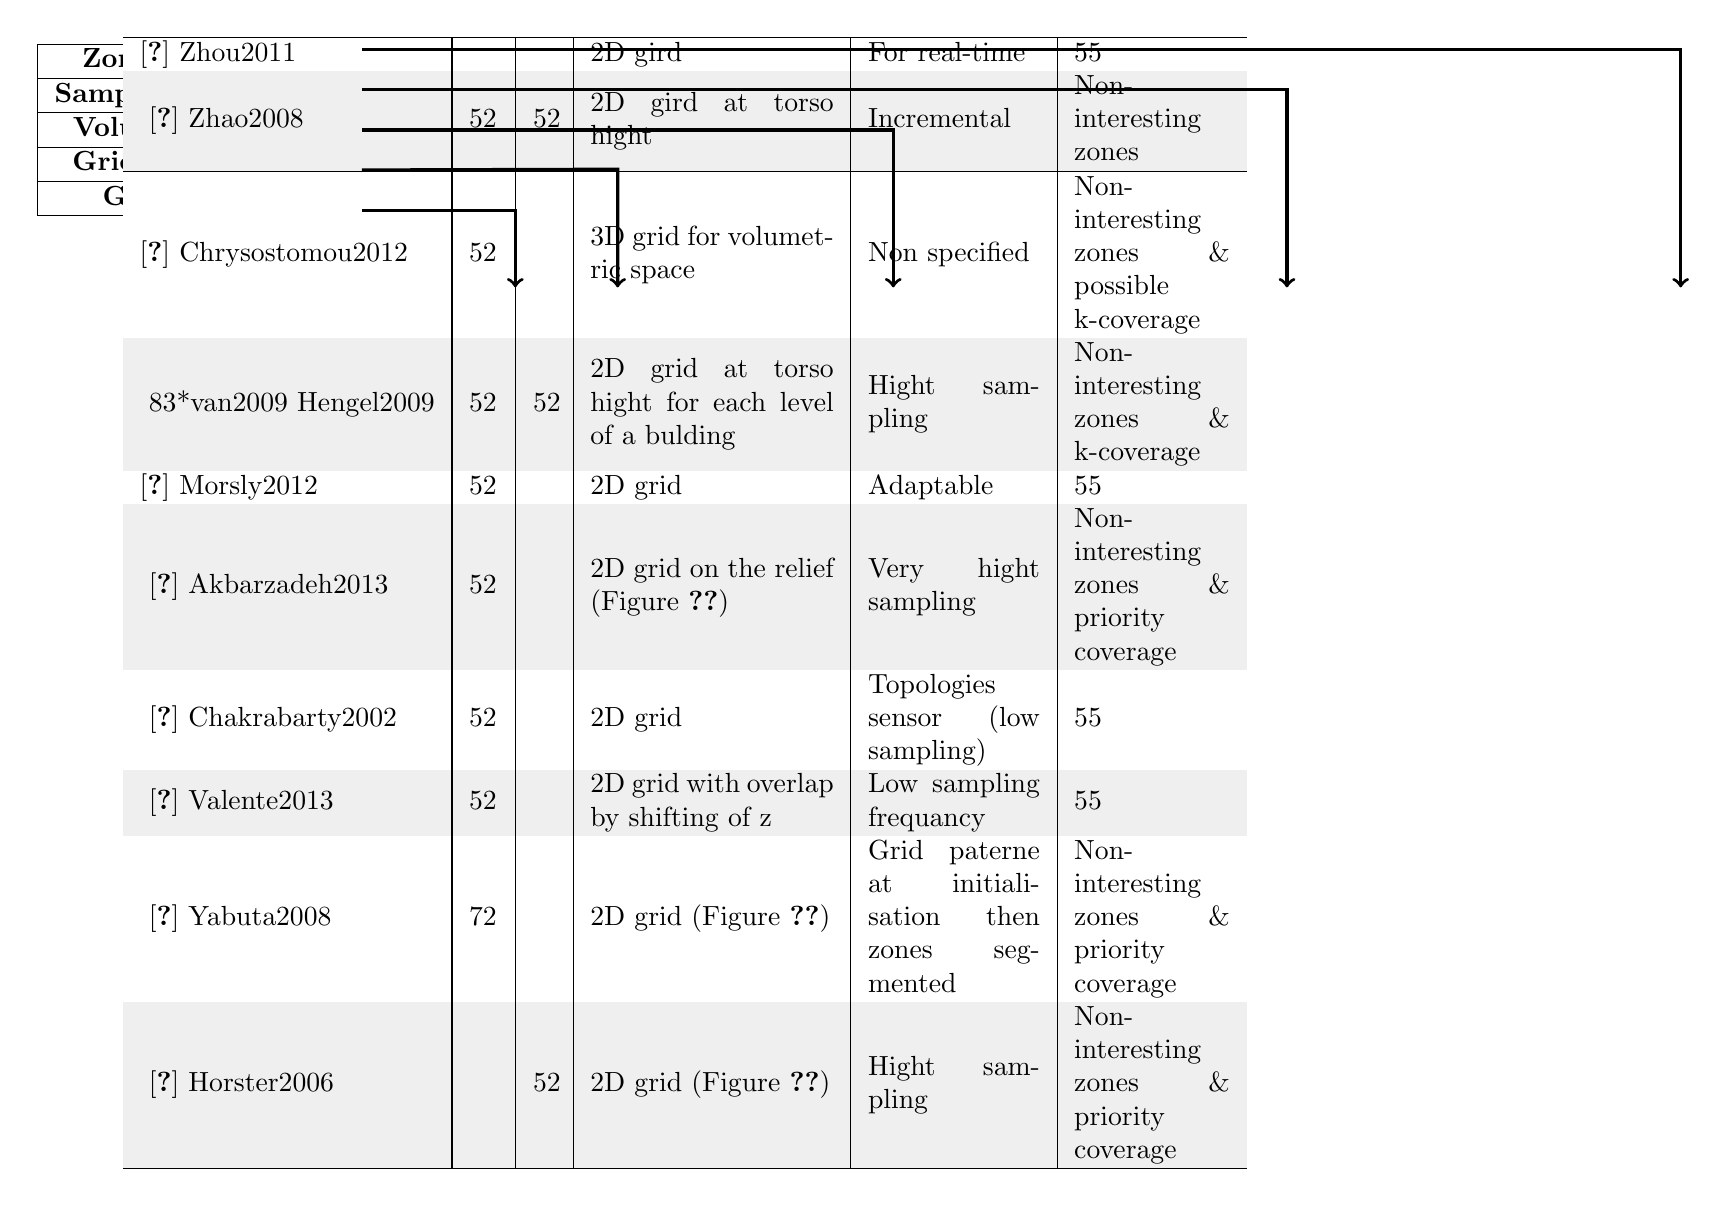
\begin{tikzpicture}[right]
\node (a) at (0,0)
{

\begin{tabular}{|c|}
\hline
  \textbf{Zone of  interest} \\ \hline
   \textbf{Sampling frequency}   \\\hline %\vdots
  \textbf{Volumetric space}  \\\hline
   \textbf{Grid randomness }\\ \hline
   \textbf{Grid pattern}  \\ \hline
\end{tabular}
};

\node[yshift=-4.789cm,xshift=-1cm] (b) at (a.south) 
{
\begin{tabular}{l | m{0.031\linewidth} | m{0.024\linewidth} | m{0.255\linewidth} | m{0.18\linewidth} | m{0.1631\linewidth} }
\hline
\toprule

\rowcolor[HTML]{FFFFFF} 
\multicolumn{1}{l|}{\cellcolor[HTML]{FFFFFF}\cite{8*zhou2011} Zhou2011}   		&	 %\ding{52} 
	 &	     & 	   				2D gird		  & For real-time    &  \ding{55} \tabularnewline    	
\rowcolor[HTML]{EFEFEF} 
\multicolumn{1}{l|}{\cellcolor[HTML]{EFEFEF} \cite{22*zhao2008} Zhao2008}  		&	  \ding{52}	 &	  \ding{52}   & 	   	2D gird at torso hight	  & Incremental	 	 &  Non-interesting zones  \tabularnewline \hline     
 \rowcolor[HTML]{FFFFFF} 
\multicolumn{1}{l|}{\cellcolor[HTML]{FFFFFF}\cite{82*chrysostomou2012} Chrysostomou2012}  &	  \ding{52}	 &	     &	3D grid for volumetric space  &  	Non specified			 &  Non-interesting zones  $\&$ possible k-coverage \tabularnewline 
\rowcolor[HTML]{EFEFEF} 
\multicolumn{1}{l|}{\cellcolor[HTML]{EFEFEF} \citep{83*van2009} Hengel2009 } 		&	  \ding{52}	 &	  \ding{52}  & 	2D grid at torso hight for each level  of a bulding  &  	Hight sampling	 & Non-interesting zones  $\&$ k-coverage	\tabularnewline 
  \rowcolor[HTML]{FFFFFF} 
\multicolumn{1}{l|}{\cellcolor[HTML]{FFFFFF}\cite{87*morsly2012} Morsly2012} 	 	&	  \ding{52}	 &  & 2D grid  &  	Adaptable	 &   \ding{55}	\tabularnewline 
\rowcolor[HTML]{EFEFEF} 
\multicolumn{1}{l|}{\cellcolor[HTML]{EFEFEF} \cite{141*akbarzadeh2013} Akbarzadeh2013 }      &	  \ding{52}	 &	     & 	2D grid on the relief (Figure \ref{fig:grilleRef141})  &  	Very hight sampling 		 &  Non-interesting zones  $\&$ priority coverage \tabularnewline 
  \rowcolor[HTML]{FFFFFF} 
\multicolumn{1}{l|}{\cellcolor[HTML]{FFFFFF} \cite{150*chakrabarty2002} Chakrabarty2002}    &	  \ding{52}	 &	     & 	  	 	2D grid		  & Topologies sensor (low sampling) & \ding{55}	\tabularnewline 
\rowcolor[HTML]{EFEFEF} 
\multicolumn{1}{l|}{\cellcolor[HTML]{EFEFEF} \cite{164*valente2013} Valente2013}       &	  \ding{52}	 	&	     & 2D grid with overlap by shifting of z  &  	Low sampling frequancy			 &	\ding{55}\tabularnewline 
   \rowcolor[HTML]{FFFFFF} 
\multicolumn{1}{l|}{\cellcolor[HTML]{FFFFFF} \cite{170*yabuta2008} Yabuta2008}         &	  \ding{72}	 & 	     &		  	2D grid (Figure \ref{fig:from170})	  & Grid paterne at initialisation then zones segmented  & Non-interesting zones  $\&$ priority coverage \tabularnewline 
\rowcolor[HTML]{EFEFEF} 
\multicolumn{1}{l|}{\cellcolor[HTML]{EFEFEF} \cite{171*horster2006}  Horster2006}   &	  	 &	  \ding{52}   & 	  	 	2D grid (Figure \ref{fig:randomGridRef171})		  &  	Hight sampling 	 	 	 &  Non-interesting zones  $\&$ priority coverage \tabularnewline \hline
   \rowcolor[HTML]{FFFFFF} 
%\multicolumn{1}{l|}{\cellcolor[HTML]{FFFFFF}\cite{174*zhang2016}  Zhang2016}    &	  \ding{52}	 	&	     & 	 	 			2D grid   & 				 &  \ding{52} \tabularnewline \hline

    	 
\end{tabular}
};
%\draw[->,ultra thick](a)--(b);
\draw [->,very thick] (4.25,1.02) -- (21,1.02) -- (21,-2);
\draw [->,very thick] (4.25,0.51) -- (16,0.51) -- (16,-2);
\draw [->,very thick] (4.25,0.0) -- (11,0.) -- (11,-2);
\draw [->,very thick] (4.25,-0.51) -- (7.5,-0.5) -- (7.5,-2);
\draw [->,very thick] (4.25,-1.02) -- (6.2,-1.02) -- (6.2,-2);

%\draw [->,very thick] (-1,0) -- (1,0) -- (1,-2);
%\draw [->,very thick] (-1,-0.5) -- (0,-0.5) -- (0,-2);
\end{tikzpicture}
 \caption{Sum-up of the grid map.}\label{tab:mapSumUp}
\end{table}	
\end{landscape}
 
\subsection{Our approach}
 Based on the designs studied, the one finally adopted is a grid $G$ as in Eq \ref{eq:Grid} with an uniform distribution following the 2D grid pattern. The grid pattern has been selected due to its facility of implementation and  flexibility to additional constraints.
  The frequency adopted is fixed depending on the size of the area, the precision required and the cameras properties. The frequency adopted has to be considered as dense (high sampling frequency).
  Also, due to the high sampling frequency, the 2D grid pattern is more appropriate choice and allows a reasonable number of points to describe a complex area. 
  The grid is placed on the floor of the area to cover. Floor is always considered as flat without relief.
  In our case, the zones of interest can be varied and may include non-interesting zones, priorities zones  and  multi-coverage. \\
  To possibly allow all these zones of interest features, the selected design of the grid is based on the formulation from the Eq:\ref{eq:PcFull}. During the experiments presented in the following  chapters, the priority zones and multi-coverage are not exploited. Consequently, the $k=1$ and $p=1$.  Although some brief tests were carried out with k-coverage and priority zone constraints. The results obtained were considered irrelevant, hence the choice to focus on constant priorities and single camera coverage for the entire area to be covered.\\
% Although, some prompt tests were carried-out with constraints of k-coverage and priority zones, the results obtained were considered irrelevant hence the choice to focus on constant priorities and single camera coverage for the entire area ($k=1$ and $p=1$).
%   The zone of interest can vary depending on the need of the experimentation, but the design chosen is flexible to apply if necessary the formulation form the Eq:\ref{eq:PcFull} with mostly $k=1$ and $p=1$, also a set $U$ is used to represent the non-interesting zone as it was presented in eq \ref{eq:setU}.

%%%%%%%%%%%%%%%%%%%%%%%%%%%%%%%%%%%%%%%%%%%%%%%%%%%%%%%%%%%%%%%%%%%%%%%%%%%%%%%%%%%%%%%%%%%%%%%%%%%%%%%%
%%%%%%%%%%%%%%%%%%%%%%%%%%%%%%%%%%%%%%%%%%%%%%%%%%%%%%%%%%%%%%%%%%%%%%%%%%%%%%%%%%%%%%%%%%%%%%%%%%%%%%%%
%%%%%%%%%%%%%%%%%%%%%%%%%%%%%%%%%%%%%%%%%%%%%%%%%%%%%%%%%%%%%%%%%%%%%%%%%%%%%%%%%%%%%%%%%%%%%%%%%%%%%%%%
\section{Camera coverage}\label{sec:CamerasCoverage}


Once the area to cover is described by the grid, the next step is to verify for each point of the grid if one or more cameras cover it, based on Eq: \ref{eq:PcFull} with $k=1$ and $p=1$.\\
To verify if each points of the grid is covered by a camera. It is primordial to discuss the camera properties and introduce the projection model.
%to talk about what is a camera, what kind of cameras are appropriate and their projection model. 

%%%%%%%%%%%%%%%%%%%%%%%%%%%%%%%%%%%%%%%%%%%%%%%%%%%%
\subsection{Camera definition}\label{sec:CamerasDefinition}

The perspective projection is often used to define a camera. The camera projection has the advantage to be anamorphic 
%The closest projection model to the human view is the perspective projection. 
Thus, the perspective projection is also the most common and more especially in the field of area coverage as presented in examples \cite{101*topcuoglu2009,33*reddy2012,8*zhou2011,82*chrysostomou2012,22*zhao2008}. Other models of camera or vision sensors can be used such as for example omnidirectional with a $360^{\circ}$ field of view \citep{43*erdem2006,150*chakrabarty2002,174*zhang2016}. 
In the following chapters ,we are only focusing on the camera perspective due to its wide use and it is also the most suitable to be embedded in UAVs for path planning. 
\begin{figure}[t!]
\begin{center}
 \minipage{0.65\textwidth}
   \includegraphics[width=\linewidth]{img/PinholeCam.png}
  \caption{Pinhole camera model.}\label{fig:cameraObscura}
  \endminipage\hfill
\end{center}
\end{figure} 
\\The pinhole or in Latin the "camera obscura" (see Figure\ref{fig:cameraObscura}) is at the origin of the geometry model for the perspective projection.\\
The pinhole model is commonly composed by a box (or  a chamber) hermetically closed to light, excepted by a small pinhole on the middle of the front side. All the ray of light reflected by the objects of the world and passing by the small hole are projected onto the back side of the box. Each ray of light passing by the hole is  projected onto a plan ( the back side of the inside box). This plan observes the reversed image of the world and can be recorded by a film or a digital sensor. 
 Due to the simplicity of the pinhole model, the calibration and camera projection estimation is simplified. To estimate the projection, only few elements has to be known:
%  Based on it, the camera projection is dependent then few parameters intrinsic (as focal length, sensor size,...) and extrinsic (as the position $x,y,z$ and orientation $\alpha,\beta,\gamma$). 
  
 
\begin{figure}[t!]
\begin{center}
\minipage{0.65\textwidth}
   \includegraphics[width=\linewidth]{img/PanTiltRoll.png}
  \caption{The rotation composed by three degrees of freedom on pan tilt roll $(\alpha,\beta,\gamma)$.}\label{fig:PanTiltRoll}
  \endminipage\hfill
  \end{center}
\end{figure}

%In fact the useful elements to define the projection of a camera perspective, can be stated as a set of parameters composed by:\\
\begin{itemize}
\item Three degrees of freedom for the camera position : $(x, y, z)$;
\item Three degrees of freedom for the camera orientation : pan, tilt, and roll angles: $(\alpha,\beta, \gamma)$ 
\item Optical parameters including: the focal length $f$ of the lens, %{the sensor size $Sw\times Sh$,
 $u_{0}$ and $v_0 $  which would be ideally in the conter of the image. $\sigma_{uv}$ represents the skew coefficient between the $x$ and the $y$ axes.
\end{itemize}
%$s$ is composed by two elements $Sw$ and $Sh$ for the size of width and height (also called  the scale factor).\\

Among the parameters of the camera, only  some of them are useful to estimate the projection. They can be formalized as a vector:
\begin{equation}\label{eq:v}
v=(x,y,z,\alpha ,\beta,\gamma,f)%,u_0,v_0,\sigma_{uv} %v=(x,y,z,\alpha ,\beta,\gamma,f,S_w\times S_h)
\end{equation}

Each elements of the vector $v$ are used to compute the camera projection on the discretized floor (the grid $G$). 
\iffalse 
To model the camera set using the precedent notation, a set $V$ composed by $N$ cameras defined by $v$ noted:
\begin{equation}\label{eq:V}
\begin{split}
V= \{v_i\} \mbox{  , } \forall i=[1;N] \mbox{ , } N\in \mathbb{N}^*
\\
\mbox{ and } v_i= (x_i,y_i,z_i,\alpha_i ,\beta_i,\gamma_i,f_i,s_i,{u_0}_i,{v_0}_i,{\sigma_{uv}}_i)
\end{split},
\end{equation}
\noindent Where $N$ is the given number of cameras in the solution. Which is also the number of cameras in the set $V$. \\
Therefore, $V$ represents a camera network and also an initial set of parameters for a camera set. $V$ can contain all the possibilities, including the non-acceptable solution(s). A non acceptable  solution will be a solution which  does not adheres the constraints of the problem. \\ 

%%%%%%%%%%%%%%%%%%%%%%%%%%%%%%%%%%%%%%%%%%%%%%%%%%%%  
  
 
    
The hole in the box is called the projection center. It is the point were each rays of light are crossing together.  \\
Based on this model, a 3D point $^CP=(^Cx,^Cy,^Cz,1)^T$ defined in the pinhole reference noted $ ^C\Re$ can be converted into a 2D point  $^rp=(^ru,^rv,1)^T$ in the sensor reference frame (back side of the box) by using  the perspective projection model $pr() $: 
\begin{equation}
^rp=(^ru,^rv)= pr(^CP) \mbox{ with } \begin{cases} u= f.\frac{^Cx}{^Cz} \\  v= f.\frac{^Cy}{^Cz} 
\end{cases} 
\end{equation}
Where $f$ is the focal length (distance between the projection center and the photosensitive sensor).
The point $^rp$ is the projected point $^CP$ on the sensor. The sensor is composed by $sw$ pixel of width and $sh$  pixel of  height. To convert the coordinate $^rp$ of p in the pixel  that means in the image reference $^i\Re$ : 
\begin{equation}
^ip=K. ^rp,
\end{equation}
Where $^ip$  is the point $p$ in the image reference composed by $(u,v) \in ^i\Re$ with $u$ and $v$  pixel coordinates. 


%Where $u_0$ and $v_0$ are the coordinate  of  the principal point of the image ( projection of the optic centre on to the image plan).  
%$k_u$ and $k_v$  are the magnification factors of the image on width and heigh. 

% resource http://ksimek.github.io/2013/08/13/intrinsic/
%https://jeux.developpez.com/tutoriels/OpenGL-ogldev/tutoriel-12-projection-perspective/
The cameras is called calibrated when the intrinsic parameters ($K$) are known.  
 The intrinsic matrix $K$ is parametrized by Hartley and Zisserman and permits to represent the properties of the camera. To design the intrinsic matrix $K$ some parts of the pinhole camera have to be defined :\\
  \begin{itemize}
  
 	\item $f$ is  the focal length. The focal length is the distance between the pinhole and the sensor (a.k.a. image plane)
  	\item $k_u et k_v$ are the magnification factors of the image on width and height ; related to the image sensor format%  les facteurs  aggrandisement de l'image 
  	\item $u_0 v_0$  are the coordinates  of  the central point of the image ( projection of the optical center on to the image plane)  %the les coordonnées de la projection du centre optique de la caméra sur le plan image 
  	%\item $s_uv$ qui traduit la non-orthogonalité potentielle des lignes et des colonnes de cellules électroniques photosensibles qui composent le capteur de la caméra. La plupart du temps, ce paramètre est négligé et prend donc une valeur nulle.\\
  	  \end{itemize}
		Once these elements are known, the matrix $K$ can be designed :
	\begin{equation}
		K=
		\begin{pmatrix}
			k_u 	& 0 	& u_0 \\
			0 		& k_v	& u_1\\
			0 		&	0	& 1
		\end{pmatrix} .
		\begin{pmatrix}
			f 		& 0 	& 0  \\
			0 		& f		& 0  \\
			0 		&	0	& 1  
		\end{pmatrix} 
	\label{eq:K}
	\end{equation}
Finally, in order to estimate the positions of a 3D point in the pinhole camera reference $^C\Re$ into the image reference $^i\Re$ 
$$
^ip=K.pr(^CP)
$$ 	  
 Parameter extrinsic (global definition ) \\
  \begin{itemize}
 	\item$R_3x3$ = la matrice de rotation permettant de passer du repère lié à l'espace de travail au repère lié à la caméra\\
 	\item$t_x t_y t_z$ = les composantes du vecteur de translation permettant de passer du repère lié à l'espace de travail au repère lié à la caméra.\\
  \end{itemize}
 %Parameter utile pour notre cas de figure \\     fig : \ref{eq:V}\\
 
!!!!! the previous section can be largely (keep the basic introduction remove to be replace by ... !!!!!
\fi
%%%%%%%%%%%%%%%%%%%%%%%%%%%%%%%%%%%%%%%%%%%%%%%%%%%%%%%%%%%%%%%%%%%%%%%%%%%%%
\subsubsection{Coverage estimation in the literature}


%To estimate the coverage of a set of camera $V$  the cameras projection of each $v_i$ has to be computed individually.
 In order to compute the camera projection onto a grid, the pinhole model is used with the parameters of the vector $v$, previously defined.\\
The detail to estimate the camera projection onto the floor, based on the pinhole model and the parameters ($v$), have been detailed numerous times such as in \cite{193*fu2014,181*wang2017,165*jiang2010}. In \cite{193*fu2014,181*wang2017,165*jiang2010}, the camera projection is used to estimate if a point $g_i$ of the grid is visible by a given camera, and that for each point of the grid. These articles handles the classic camera projection, with  the six Degrees of Freedom (DoF) in \citep{193*fu2014} and five DoF in \citep{181*wang2017}). Both are used to estimate the 2D projection of the camera onto the floor (as in Figure \ref{fig:cam_projOnGrid}). \\
In  \citep{193*fu2014}, the camera projection have been computed for several rotations for all the DoF. In this case, the projection can have numerous shapes (mostly parallelogram shapes).\\
In \citep{181*wang2017}, the model of camera projection begins to be simplified by assuming some fixed parameters. The fixed parameters allows more efficient estimation, by economizing part of projection computation of the camera at each time. The fixed parameters allows the pre-estimation  all of part of the shape.  \\
In \citep{165*jiang2010}, the model of camera projection is used to compute one time for a fixed pan and roll in order to have a coverage estimation usage in a 2D map. The camera projection is finally simplified by using a kind of triangular shape.\\
To go further, other models and formulations inspired by the pinhole model were proposed \cite{87*morsly2012,141*akbarzadeh2013,146*li2011,194*fu2010}. These models are inherited from the camera projection and adapted to fit each relative problems. \\
In \cite{87*morsly2012,194*fu2010}, the camera is considered placed on the floor with a fixed pan (with the viewing direction almost parallel to the floor). Therefore, the camera projection is simplified by an isosceles triangle where the shape depends on the focal length.\\
In \citep{141*akbarzadeh2013}, the camera projection is also simplified to obtain a kind of isosceles triangle shape while considering the depth of view of the camera. In this case, the  camera projection has a "piece of pie" shape. \\
In \citep{146*li2011}, thanks to a fixed pan and focal length, the camera projection is simplified to have a rectangular projection onto the ground. The sweep is designed consequently to the size of the camera projection, in order to minimize the overlap and have full coverage of the area.  

One of the common point of the following papers  \cite{87*morsly2012,141*akbarzadeh2013,146*li2011,194*fu2010,22*zhao2008,33*reddy2012,193*fu2014,181*wang2017,165*jiang2010}    is the computation of a camera projection onto a grid. 
The computation of the function $f()$ which has to estimate whether a point $g_i$ of the grid is covered by a cameras $v_j$ of the network,  is not considered as really greedy (in time). But the coverage estimation using $f(g_i,v_j)$ for a point $g_i$ by a camera $v_j$ requires to be performed for each points of the grid and for each cameras of the network in order to estimate properly the complete area coverage.
	\begin{equation} \label{eq:sum sum v g}
		\mbox{Coverage Rate}=\sum_{i=1}^{m}\sum_{j=1}^{n}f( v_j,g_i)
	\end{equation} % for Eq Cf:87* 150*  171* voir 165*
Where $n$, the number of cameras ($v_j$) in the network; $m$ the number of point in the grid ($g_i$).  \\
%%%%%%%%%%%%%%%%%% object oclution%%%%%%%%%%%%
The solutions proposed until now to estimate the camera projection onto the grid (as in Equation \ref{eq:sum sum v g})  do not take into account the occlusion made by potential obstacles.
The occlusion  projected by  the obstacles requires to be taken into account depending on the camera projection.
 %Some of them as \citep{165*jiang2010,181*wang2017,141*akbarzadeh2013} include the object occlusion. 
 To detected the part of the area occluded by an object, the solution commonly proposed (as is well explain in  \citep{181*wang2017}) is to check the line made between a point covered ($g_i \in Pc$) and its camera. If this line is intersected by at least by one object in the scene, the point $g_i$ cannot be considered anymore as covered. 
%  Despite the simplicity of the computation numerous operation have to be done to compute the camera projection onto the floor. \\

To take into account the potential occlusion by an obstacle $Obj_l$, the Equation \ref{eq:sum sum v g} can be extended : 
	\begin{equation}
		 \mbox{Coverage Rate}=\sum_{l=1}^{k}\sum_{j=1}^{m}\sum_{i=1}^{n}f( v_i,g_j,Obj_l)
	\end{equation} 
 
The function $f(...)$, in charge of computing a camera projection, will be called for each camera, each point of the grid and each obstacle, in order to evaluate the complete coverage of the area (with the occluded part). This numerous calls will greatly increase the computation time of the coverage. It is even more affected when numerous camera projections requires to be computed at each turn of a long optimization process.\\
In these conditions, the efficiency of the function $f(...)$ computing the coverage estimation, is primordial due to the repeated calls. 
%%%%%%%%
%%%%%%%%%%%%%%%%%%%%%%%%%%%%%%%%%%%%%%%%%%%%%%%%%%%%%%%%%%%%%%%%%%%%%%%%%%%%%%%%%%%%%%%%%%%%%%%%%%%
%\begin{landscape}	
%	\begin{table}[]
%\centering
%\caption{Sum-up ref}
%\label{tab:sum-up1}
% %              ref           |x|y |z|       tilt| |focal  coverage     nmb   
%\begin{tabular}{@{}l|p{2.4cm}    l  p{0.62cm}lp{1.3cm}p{1.57cm}p{1.5cm}p{1.6cm}p{1.3cm}p{1.2cm}@{}}
%\toprule
%\multicolumn{1}{|l|}{\textbf{Ref}}   & \multicolumn{1}{l|}{Y}              & \multicolumn{1}{l|}{Pan} & \multicolumn{1}{l|}{Tilt} & \multicolumn{1}{l|}{Roll} & \multicolumn{1}{l|}{\begin{tabular}[c]{@{}p{1.55cm}@{}}Coverage\\  room\end{tabular}} & \multicolumn{1}{l|}{\begin{tabular}[c]{@{}l@{}}Number\\ of \\ cameras\end{tabular}} & \begin{tabular}[c]{@{}l@{}}Secondary objectives \\ and constraints\end{tabular} &                      &               \multicolumn{1}{l|}{} \\ \midrule
%\rowcolor[HTML]{FFFFFF} 
%\citep{193*fu2014}   Fu 2014                                                                                                                                    & \ding{52}                                   &  \ding{52}                        & 0                         & 0                                                       & 2D                                                                                      & $\approx 10                                                                        $                                                           & barrier coverage                                                               & conection dependance &                                     \\
%\rowcolor[HTML]{EFEFEF} 
%\cite{181*wang2017}    Wang 2017                                                                                                          & 0                        & 0                         & 0                                                       & 2D                                                                                      & $\approx 600                                                                        $ & resolution                                                                     & tracking             &                                     \\
%\rowcolor[HTML]{FFFFFF} 
%\citep{165*jiang2010}   jiang 2010                                                                                                                                    & \ding{52}                                   &  \ding{52}                        & 0                         & 0                                                       & 2D                                                                                      & $\approx 10                                                                        $                                                           & barrier coverage                                                               & conection dependance &                                     \\
%\rowcolor[HTML]{EFEFEF} 
%\citep{141*akbarzadeh2013}  Akbarzadeh 2013                                                  &  \ding{52}                                   &  \ding{52}                        &  \ding{52}                         & 0                         &  \ding{52} & 2D                                                                                      & 9 to 15                                                                           & region of interest                                                              & big area             &                                     \\ 
%\rowcolor[HTML]{FFFFFF} 
%\citep{87*morsly2012}   Morsly 2012                                                                                                                    & \ding{52}                                   &  \ding{52}                        & 0                         & 0                                                     & 2D                                                                                      & $\approx 10                                                                        $                                                           & barrier coverage                                                               & conection dependance &                                     \\
%\rowcolor[HTML]{EFEFEF} 
%\cite{146*li2011}    Li 2011                             & 0                        & 0                         & 0                                                       & 2D                                                                                      & $\approx 600                                                                        $ & resolution                                                                     & tracking             &                                     \\ 
%\rowcolor[HTML]{FFFFFF} 
%\citep{194*fu2010}  Fu 2010                                                       & \ding{52}                                   &  \ding{52}                        & 0                         & 0                                                        & 2D                                                                                      & $\approx 10                                                                        $                                                           & barrier coverage                                                               & conection dependance &                                     \\
%\rowcolor[HTML]{EFEFEF} 
%\citep{22*zhao2008}  Zhao 2008                                         &  \ding{52}                         & 0                         &  \ding{52} & 2D                                                                                      & 9 to 15                                                                           & region of interest                                                              & big area             &                                     \\ 
%\rowcolor[HTML]{FFFFFF} 
%\citep{33*reddy2012}  Reddy 2012                   &  \ding{52}                        & 0                         & 0                         & fix                               & 2D                                                                                      & $\approx 10                                                                        $                                                           & barrier coverage                                                               & conection dependance &                                     \\\bottomrule
%\end{tabular}
%\end{table}
%\end{landscape}	
%%%%%%%%%%%%%%%%%%%%%%%%%%%%%%%%%%%%%%%%%%%%%%%%%%%%%%%%%%%%%%%%%%%%%%%%%%%%%%%%%%%%%%%%%%%%%%%%%%%

\subsubsection{Coverage estimation optimization} \label{sec:coverageEstimation}
To design an efficient cost function, it is necessary to reduce the  computation time and estimate the covered area . %A good estimation of the covered area  is primordial for the optimisation process. 
  The camera projection model has to be simplified with some basic assumptions relative to the problems.\\
Considering our case, a camera is fixed on a UAV with a viewing direction orthogonal to the ground (without any rotation in $\alpha$ pan and $\beta$ tilt). 
In this model, the camera projection is always a rectangle as shown in Figure \ref{fig:cam_proj}. In fact, the camera is  placed on a UAV and have a direct view onto the ground. The viewing direction of the cameras is  perpendicular to the floor, implying the rectangle projection.
The area covered  by the camera is defined by the rectangle defined by $Wr\times Hr$ 
It is possible to compute the size of the covered rectangle for a given altitude by one camera, based on these given parameters. 
%To compute the size of the projected rectangle the focal length $f$, the altitude of the cameras $A$ and the sensor size $Sw\times Sh$ is required. 
%Especially the focal length $f$, the altitude of the cameras $A$ and the sensor size $Sw\times Sh$. \\

%The altitude is the distance between the grid and the cameras, in the simple case $A$ is considered to be equal to $z$, when the grid is on the floor.  \\
Based on the useful parameters from the camera $(f ,S_w\times S_h ,z)$, the computation estimating the size of a camera projection ($Wr$,$Hr$) is :

%\begin{equation}
%s= [Sw ; Sh]  %\mbox{   } Sw,Sh \in \mathbb{N} 
%\end{equation}
%
%\noindent Where $Sw$, sensor size width. \\
%Where $Sh$, sensor size height.

%Where $\eta$, $\upsilon$ are the horizontal and vertical camera fields of view.\\
%Estimating the width and height of the rectangle projected on the ground depend on the altitude $A$ :
%	\begin{equation}\label{eq:WrHr1}
%		\begin{split}
%    		Wr= 2\times A\times\tan \frac{\eta}{2}
%    	    \\
%    	    Hr= 2\times A\times\tan \frac{\upsilon}{2}
%    	 \end{split}
%	\end{equation} 
	
	
	\begin{equation} \label{eq:WrHr1}
	\begin{split}
			Wr=(\frac{1}{f} . S_w).z\\
			Hr=(\frac{1}{f} . S_h).z
     \end{split} 
	\end{equation}
	
	\begin{figure*}[t!]
		\centering
		\minipage{0.85\textwidth}
  		\includegraphics[width=\linewidth]{img/CamProject1Bis.png}
  
 	 	\endminipage\hfill\caption{Camera projection onto a grid. The grid is placed on the floor to discretize 	the area covered.}\label{fig:cam_proj}
	\end{figure*}

%Therefore, the size of the rectangle projected onto the floor is $(Wr,Hr)$ for the width and height. The values of $Wr$ and $Hr$ are directly linked to the altitude of the camera. 


%In the simple case and in the initialization, $A$ is equal to $z$ and $z$ is selected in a range given by the UAV or the user. \\
%Once the couple $(Wr,Hr)$ as been computed for a $A=z$ it is easier to change the altitude of the camera. The rectangle projection will be affected in proportion.
%	\begin{equation}\label{eq:A.coef}
%		\begin{split}
% 		   	f(A)= (Wr,Hr) \text{ based on eq \ref{eq:WrHr1}}\\
%    		f(A.Coef)=f(z)= (Wr.Coef,Hr.Coef)      
%    	 \end{split} 
%	\end{equation}
%Therefore, to any altitude $z$ is existing $A.Coef$ where the size of the camera projection onto the floor is $(Wr.coef, Hr.coef)$. Thanks to this the eq: \ref{eq:etaUpsilon} and eq: \ref{eq:WrHr1} have to be compute once  for a given focal length $f$ and sensor $s$ with an simple $A=z$. Adding simple $Coef$ the size of camera projection can be easily simplified in order to limit the useless computation (only 2 multiplication instead then equation \ref{fig:cam_proj} and \ref{eq:etaUpsilon}.

When $f$ represents the focal length, $z$ the altitude of the cameras and  $S_w$, $S_h$ the sensor size.
%The model of camera projection is greatly simplified by the UAV assumption (fixed pan, tilt and focal length).
Thanks to this model of camera projection drawing a simple rectangle, the size of the rectangle projection is directly related to the altitude. The altitude is assuming to be a coefficient of the Equation \ref{eq:WrHr1}\\
%The simplification by modelling all the cameras with a fix orientation and same ability (in order to have a rectangle projection onto the ground) 
All these simplifications helps the cost function to be fast and efficient.  In fact, in the Equation \ref{eq:WrHr1}, the focal length parameters and the sensor size are fixed and do not need to be recomputed for each camera position only the altitude $A$ has to be updated.\\

\subsection{Parameters to optimization }\label{sec:parameterToOptimize}
% en raison de    ref 191*
By simplification presented previously, the parameter vector (see Equation \ref{eq:v}) can be reduced.
The computation of one camera projection onto a grid (as in Section \ref{sec:GridMap} and the camera are placed in altitude with a viewing direction orthogonal to the floor. Based on the Equation \ref{eq:WrHr1},
just few parameters are necessary as shown in Equation \ref{eq:WrHr1}. Thanks to the proposed assumption,  Equation \ref{eq:v} can be reduced by keeping only the position of the camera $(x,y,z)$ and the roll ($\gamma)$ as:
	\begin{equation}\label{eq:v2}
		v=(x,y,z,\gamma ) 
	\end{equation}

In our case, the roll $\gamma$ can take two different states, portrait or landscape with respectively a rotation of $0^\circ$ or $90^\circ$.
Reducing the number of  parameters, passing from the equation \ref{eq:v} and \ref{eq:v2} reduces the number of parameters to optimize. 

 % The reduction of the number of parameters will greatly affect the optimisation process.
 %Indeed, in addition to reduce the time computation, this simplification reduce the number of parameters to optimize.   

Until now, the camera projection estimation was addressed with only one camera. But we want to compute the coverage for a camera set. 
The solution is based on the previous estimation for the camera projection but adapts to the location of each cameras by positioning the rectangle projection to have the center at the $x$ and $y$ position and compute the occupation grid.

In order to gain a bit of time, each point of the grid already covered by a camera are not tested for the next cameras. %This small modification will impact positively the computation time for the coverage estimation of a network of cameras. 
Which means that in the equation \ref{eq:sum sum v g}, the value of $m$ decrease as $i$ increase. More exactly the size of $m$ decrease as the area coverage increase.  


\subparagraph{Parameters representation \\}

To represent the problem, we need a set of cameras. The previous notation can be extended to have a set $V$ of $n$ cameras defined according to:

\begin{equation}\label{eq:V}
		\begin{split}
			V= {v_1,v_2,...,v_n} \mbox{  , } n\in \mathbb{N}^*
				\\
			\mbox{ with } v_i= (x_i,y_i,z_i,\gamma_i)
		\end{split}
	\end{equation}
	
%	\begin{equation}\label{eq:V}
%		\begin{split}
%			V= \{v_i\} \mbox{  , } \forall i=[1;n] \mbox{ , } n\in \mathbb{N}^*
%				\\
%			\mbox{ and } v_i= (x_i,y_i,z_i,\gamma_i)
%		\end{split}
%	\end{equation}
\noindent Where $n$ is the given number of cameras in the network. The coordinates of a camera $v_i$ which are the $i$th camera of the network is defined  with $x_i, y_i, z_i,$ in a given room and $\gamma_i$ the roll rotation (portrait or landscape). The not contained parameters in $V$ and used to compute the cameras projection are  identical for all the set $V$, and are fixed at the beginning of the optimization.\\
Therefore, $V$ represents a solution. $V$ contains all individual positions and orientations of the camera set for a predefined focal length, sensor size and related map depending on the problem.% wish also include the potential constraint as  some restriction on the map.\\
 Obviously, all the solutions $V$ are not a "possible solution" for our problem. Some solutions $V$ does not complies the set of constraints noted $E$. E represents the set of constraints ( the set E is defined  in details later). 

In addition, the solution $V$ should comply a set of constraints  $E$ (see Eq.\ref{eq:Vs}). Among the constraints, few of them were already discussed, as the occlusion, the map restriction, the k-coverage, or some constraints more specific to the problems (as shown in chapter \ref{chap:stateOfTheArt}).\\
 The "possible solution" $Vs$ must take in consideration with the set $E$ as :

%\begin{equation}\label{eq:Vs}
%Vs=V \mbox{ , iff } E(V)=\begin{cases} 1 & \mbox{iff } E_i(V)=1 \mbox{ , with } i=1...Nc \\ 0, & \mbox{otherwise} 
%\end{cases} 
%\end{equation}
 \begin{align}\label{eq:Vs}
Vs=V \mbox{ , iff } E(V)= \begin{cases} 1, & \mbox{iff } E_i(v)=1 \mbox{ , with } i=1...Nc \\ 0, & \mbox{otherwise}  \end{cases}
%\\ G'=G-U \mbox{ ,    }  \mbox{ }U= \{ g_i | g_i \in G, g_i \mbox{ are the non intresting points} \}
\end{align}

Where $E_i(V)$ is the function applied to verify  the $i$th constraint of the set $E$ on the solution $V$. $Nc$ is the number of constraints necessary to be satisfied to obtain an acceptable solution.
Among all the possible combinations of parameters $V$, only the one intersecting the set of constraints $E$ is a possible solution.  If we are considering  all the $V$ and all the $E$ as two subsets, $Vs$ is defined as $Vs=V\subset E$. 

The problem of monitoring an area and more specifically the problem of area coverage may contain many constraints depending of the environment and the context. As for example: the room shape, minimizing  the altitude,  have the best resolution, orientation of the camera, the possible occlusion,... All these constraints are included in the set $E$. 
The constraints requires to be defined depending on the problem and the goal.

\section{Cost Function}
The cost function has to evaluate the quality of a given solution. To estimate the quality of a solution one of the main criteria is the coverage rate. The previous section was focused on the computation of the coverage rate. \\
To create an efficient cost function, other criterion has to be taken in to account as constraints.  
 To establish the cost function, a list constraints require to be established. Each constraint of this list does not have the same importance. In order to split the constraints depending on their respective impacts on the problem, two types of constraints are introduced in the  following sections before discussion.
  

\subsection{Constraint list}\label{sec:constraint}

%Make the exhaustive list of all the constraints for the problem of cameras positioning is not really interesting and almost impossible.
 The constraints can be numerous and depends mainly on the problem formulation and the context. Like that, few of them were briefly introduced in the previous section as in chapter \ref{chap:stateOfTheArt} and section \ref{sec:coverageEstimation},... This part is focused on the list of the constraints used in our case and detail their design.

%The constraint considered in this work are : 
%\begin{itemize}
%	\item Fix number of the cameras.
%	\item Fix parameters of the camera.
%	\item No rotation  on  $\alpha$ and $\beta$ (pan and tilt).
%	\item Possible fix altitude.
%	\item Altitude boundary (not too hight, not too low).  	
%	\item The map boundary (rigid rectangle).  
%	\item Non rectangles map with possible holes.
%	\item To have some fix cameras in the set. 
%	\item The resolution.\\
%
%\end{itemize} 
\subparagraph{Fixed number of the cameras}
One of the first constraint represents the establishment of number of cameras. This constraint, as some others (detailed latter), are  useful to simplify and restrict the possibility of the problem. This constraint allow us to focus on the fine optimization (as in \citep{22*zhao2008} where both are tested). The number of cameras is fixed at the beginning of the optimization and no more camera will be added during the optimization process.  

\subparagraph{Fixed parameters of camera and no rotations}
Fixed parameters of the cameras and no rotations ($\alpha$ and $\beta$) has been introduced previously (section \ref{sec:parameterToOptimize}). These constraints imposed by the use of an UAV are also an advantage for the optimization by simplifying the coverage estimation and limit the number of parameters to optimize. The parameters are fixed at each beginning of the optimization. Thanks to this constraint the optimization  has to focus on the precise  cameras positioning.

\subparagraph{Fixed altitude}
 The fixed altitude is a constraint established in order to limit the number of parameters to optimize. The usage of such constraint is linked to the reduction of the difficulty by reducing the possible search space (see section \ref{sec:OptimizationComplexity}). It is also useful for other assumptions, like a camera on the celling or for a submarine  \cite{66*galceran2013}. This constraint is an optional constraint and is not always used in the experiments presented in the following sections.   

\subparagraph{The altitude boundaries}\label{sec:altitudeBoundary}
 When the altitude is not fixed, some limits must be chosen to avoid the extremely high and low altitudes. The highest altitudes will be fixed depending on the UAV ability and other restrictions as the legislation requires it. The lowest altitude has to be fixed for the safety of the users under the UAV.  
In practice the  altitude boundaries are defined with an interval:
 \begin{equation}\label{eq:boundaryZ}
   \inf z\leq z\leq \sup z  
 \end{equation} 
 Where $\sup A$ is the maximal altitude of the camera and $\inf A$ the minimum altitude. $A$ is the altitude between the camera and the grid. %$A$ is the fix altitude of a camera where the camera projection has been computed with $A=z$ with only $coef$ vary as introduced in Equation \ref{eq:A.coef}. 
 
 \subparagraph{The map boundaries} \label{sec:MapBoundaries}
The map boundaries represent a constraint similar to the altitude boundary. Despite the shape of an area to cover, some maximum boundaries can be established. In fact, for any shape, as complex as it is, it may be possible to encapsulate it inside a rectangle. The rectangle map boundary is defined by a width $W$ and height $H$. The boundaries on $x$ and $y$ are:
 \begin{equation}
  \begin{array}{lcl}
  	0\leq x\leq W \\
  	 0\leq y\leq H 
  \end{array} 
 \end{equation}  
 
By associating the altitude boundaries (from Eq\ref{eq:boundaryZ}), cubic boundaries limits the position of the camera in the three dimensional spaces. 
\begin{equation}\label{eq:3dBoundary}
  \begin{array}{lclcl}
  	0\leq x\leq W \\ 0\leq y\leq H  \\ \inf z\leq z\leq \sup z  
  \end{array} 
 \end{equation} 
 
 \subparagraph{Non rectangle map with possible holes} \label{subPara:MapConstraintAndObstacle}
The map to cover can be much more complex than a simple rectangle and may take any shape with can be composed by holes. The Figure \ref{fig:boundaryMap} illustrates the map complexity.% The black part of the map are the zone with are out. That mean these sub-parts have not interest to be covered.
 \begin{figure}[t!]
 \begin{center}
\minipage{0.85\textwidth}
   \includegraphics[width=\linewidth]{img/BoundaryMap2.png}
  \caption{Map to cover with the map boundaries in red (W and H size) in black. The sub-part have no interest to  be covered.   }\label{fig:boundaryMap}
  \endminipage\hfill
  \end{center}
\end{figure}
To take into account the complex shape map % the gird has been designed with removing some of this points.
The grid $G$ is reduced in order to keep only the points in the white sub-part. In the example (see Figure \ref{fig:boundaryMap}), each white pixel of the map is a point of the grid to cover. 
Concretely this implementation by using a grid map has some advantages such as  the flexibility of the grid customization . \\
%Among the advantage, the flexibility of the grid customization. 
In addition, it allows the optimization to test some exotic solutions, as allowing the camera position on the black sub-part or bordering the boundaries. Obviously, the exotic solution with a camera position on the black side does not increase the coverage rate  but with a correct converge, the camera are not  covering the black sub-part of the map (or small part of it). The interest of leaving this freedom to the optimization is double. First, it controls the quality of the the solution obtained,. Secondly, the variety introduced during the exploration of the black sub-part of the map can be advantageous. 

%
%\subparagraph{Some fix cameras in the set}
%Having some fix cameras position in the set of cameras, is an optional constraint. This allows to have few manual cameras position from an user or other algorithms.
%One case can be to have some specific area as the entrance where have to be surveyed by a cameras dedicated to.  
%To implement this constraint the solution applied during the experiments (presented later) is to adapt the map by removing the point of the grid $G$ cover by the sub-set of fix cameras (as if these points of the grid was covered).

\subparagraph{Resolution}
The resolution of the images is related to the sensor size (in px) and the distance between the camera and the object. In our case, the sensor size is dependent on the properties of the camera mounted on the UAV.% and the object filmed is the floor of the area to cover.
 The distance between the camera and the floor (or the object) is the altitude as  defined in the Section \ref{sec:altitudeBoundary}. \\
 The resolution constraint has to maximize the resolution. In order to maximize the resolution during the optimization, the altitude criteria is modified in order to be as low as possible.\\
Considering only the minimization of the average altitude of the cameras is harmful for the coverage.
Consequently, during the optimization process, a trade-off between the altitude (with the related resolution) and the coverage rate have to be deduced.
 The altitude of the cameras  has to be  minimized, the average of the altitude is used as an index to estimate the resolution. %($\min{\frac{\sum^n_{i=1}{z_i}}{n}}$ )
 In order to manage this trade off, the average altitude of the cameras is included in the cost function  and has to be minimized (see section  \ref{sec:costFun}).  \\
 
\subsection{Constraint types} \label{sec:ConstraintTypesSoftHard}
 
Among the constraints listed, different priorities and restrictions exists. Indeed the constraints can be classified depending on their priorities and impact on the problems. The constraint classes are considered mostly as hard or soft constraints. %The two sub-class are the hard constraint and the soft constrain  presented in the following paragrapher.

\subparagraph{Hard Constraint}
 %Some of the constraints presented are called "Hard constraint". \\
 Hard constraints limits the possible solution by do not allowing the solution which does not respect it. These hard constraints are directly used during the optimization process to prohibit any solution to be out of these boundaries. These hard constraints are integrated in the optimization process in order to not generate a solution which does not complies it. Consequently the hard constraints may slow down the generation of the individuals due to the specific generation and required test.\\ 
 For example, the 3D boundary as defined in Equation \ref{eq:3dBoundary} is a hard constraint. Improving that, each camera must be inside the 3D boundary.\\ %Otherwise  if one of the camera are out all the solution must be rejected. 
 
 \subparagraph{Soft Constraint} 
 %In the other case, some constraint can be considered as "Soft Constraint".\\ 
 The soft constraints represents the minimization of a set of errors. 
A solution that does not fully respects the soft constraint can be considered as acceptable if the
% If a soft constraint is not fully respected the solution can be considered as acceptable and this small
 amount of errors does not affect greatly the final answer. The soft constraint is assimilated to acceptable error. \\
 The soft constraint leaves the possibility during the optimization process to allow some mistakes in order to learn about it.  
 If the soft constraint is noted $\epsilon$ and the hard constraint is noted $ \varepsilon '$, the constraint set is $E=\epsilon+\varepsilon'$.\\
 
% \begin{equation}
% 	\max f(Vs) -\epsilon  \mbox{  } \forall Vs \subset \varepsilon'
% \end{equation}
  \begin{equation}\label{eq:constraintEpsilon}
 	\max f(Vs) - \min \epsilon  \mbox{  } \forall Vs \subset \varepsilon'
 \end{equation}
 
The objective is to maximize the coverage of a set of cameras ($f(Vs)$) with respect the hard constraints $\varepsilon'$ and minimize the error from the soft constraints $\epsilon$.
Concretely, the soft constraints are commonly integrated in the Cost Function as can be the resolution or  the  complex shape of the map thanks to the grid design. 


\subsection{The cost function implementation} \label{sec:costFun}

The cost function has for mission to estimate the quality of an answer. In our case, an answer is the position  of a camera set. The cost function is essential in the process of optimization as it was introduced in the Section \ref{sec:CostFunctionGA}.

The cost function needs to estimate the area covered by a camera set. In order to do that, the area is discretized by a grid as explained in Section \ref{sec:Grid}. \\
The grid customization permits to introduce some of the soft constraints such as the complex shape of the map by removing the points out of the area to cover.  \\
The grid modification  allows the camera positions to cover the area already covered and removed from the grid. The consequence of it are the reduction of the coverage rate possibility. The optimization have to minimize this error.

To evaluate the coverage of a camera set, it is essential to estimate the cameras projection of each, as detailed in the Section \ref{sec:CamerasDefinition}. The area cover by the $j$-th camera is noted as in Equation \ref{eq:PciK} (where $Pc\in G$). By iterations, for each camera of the set, the full area coverage is computed (as Equation\ref{eq:sum sum v g}). 

Based on the previous statements, the simplest cost function is the coverage estimation.
\begin{equation}\label{eq:CostFBase}
C(Vs) =  \frac{\sum_{i=1}^n{B^{(k,p)}(G')} }{m}   
\end{equation}
Where $n$ is the number of cameras,
$m$ represents the number of points needed to describe the grid $G$ (as in Equation \ref{eq:Grid}), $Vs$ is the solution with respect to the hard constraints.
The cost function $C(Vs)$ gives the quality of the solution $Vs$.

This version of the cost function $C(Vs)$ does not take into account the resolution constraints. The resolution is  strongly linked to the camera altitude $z$ (as show in Section \ref{sec:altitudeBoundary}).
 A criteria must be added in the cost function formula of the Equation \ref{eq:CostFBase}. The average of the altitude $z$ is used and have to be included in the cost function.
 \begin{equation}\label{eq:CostFResolutionPart1}
\overline{z}= \frac{\sum_{i=1}^n z_i}{n}     
\end{equation}

 If the resolution is strongly related to the altitude, the average of it $\overline{z}$ can be considered as a part of the soft constraints ($\epsilon$)  in the Equation \ref{eq:constraintEpsilon} and the Equation \ref{eq:CostFBase} and may be updated as : 
 
 \begin{equation}\label{eq:CostFResBase}
C =  \frac{\sum_{i=1}^n {B^{(k,p)}(G')}}{m}  - \frac{\sum_{i=1}^n z_i}{n}     
\end{equation}
 
The Equation \ref{eq:CostFResBase} is used in the cost function to add the resolution constraint. Consequently, the optimization  tries to minimize the average altitude and maximize the coverage with no priority. Concretely, by just applying this Equation  \ref{eq:CostFResBase}, the optimization will first minimize the average altitude by positioning all the cameras at the minimum altitude (with respect to the hard constraint of altitude boundary) and in second time try to maximize the position (on $x$ and $y$) of the cameras. 

In order to have a priority  between the coverage and the altitude, a weight has to be established on the Equation \ref{eq:CostFResBase}. The weight requires to be chosen carefully.
The weight has to be auto-adaptable depending on area covered in order to give more priority to the coverage when the coverage rate is low and add importance to the resolution when the area is already well covered. The coverage have to remains the priority, the resolution must be optimized in a second time.
The best solution, is to link the weight of the resolution criteria with the coverage rate.

\begin{equation}\label{eq:CostFResPondere}
  \sigma \times \sum_{i=1}^n {B^{(k,p)}(G')} \times \frac{\sum_{i=1}^n z_i}{n}     
\end{equation}
Where $\sigma$ is a weighting coefficient at 0.06 to reduce the priority on the resolution criteria. 
Based on it, the final cost function is: 

\begin{equation}\label{eq:CostF}
C(Vs) =  \frac{\sum_{i=1}^n{B^{(k,p)}(G')}  - \sigma  \times \sum_{i=1}^n {B^{(k,p)}(G')} \times \frac{\sum_{i=1}^n z_i}{n}  }{m}   
\end{equation}

Thanks to this formula, a proposed answer $Vs$ can be evaluated and returns the quality of the solution for the problem of the coverage maximization and the minimization of the altitude in a second time. The cost function integrates all the soft constraints either by the design of the grid or by the formula of the cost function $C(...)$.

The cost function presented here is the final version; but the building of it was an incremental work and numerous version was tested in terms of weights, priorities, and constraints. The one presented here is the most balanced.\\ 
Despite that, some of the works  presented in the following sections are made with the basic cost function from the Equation \ref{eq:CostFBase}. In this case, the element which composes $v$ can be reduced as only $v=(x,y,\gamma)$ depending on the need of the experimentation.\\

The final and complete cost function $C(Vs)$ have as input a vector $Vs$ which is composed of all the cameras position and orientation belonging to the network. It is also composed by the map of the area to cover. Where $G$ includes the soft constraints such as the room shape. The constraint of resolution is added by using the average altitude in the equation \ref{eq:CostF}.
The value returned by the cost function $C(Vs)$ is the quality of a solution to our problems of coverage using an UAV.






%%The use of an UAV to cover an area allow the simplification of coverage computation as well as the numbers of parameters to optimize.
%% !!!!
%%Thanks to the simplification of the problem due to the used of an uav the parameters to optimize can be reduced. (as in eq: \ref{eq:v}
%%Thanks to the simplification the element to optimize for an efficient coverage can be limited to pass from Eq. (\ref{eq:v}) to  Eq.(\ref{eq:v2}) as shown: 
%%\begin{equation}\label{eq:v2}
%%v=(x,y,A,\gamma )
%%\end{equation}
 %%%%%%%%%%%%%%%%%%%%%%%%%%%%%%%%%%%%%%%%%%%%%%%%%fin de la camera pin hole explication%%%%%%%%%%%%%%%%%%%%%%%%%%%%%%%%%%%%%%%%%%%%%%%%%%%%%%%%%  
%    
%In the following part a vision sensor is employ to acquire the image of area to control. The vision sensor may be a common camera with different parameter as:
% \begin{itemize}
% \item Every camera has a position  in  $(x, y, z)$;
% \item Every camera  has an orientation composing to 3 degrees of freedom  pan$(\alpha$),  tilt$(\beta)$, roll$(\gamma)$, see Figure \ref{fig:PanTiltRoll}.
% \item Every camera have different optical parameters and the helpful to take in consideration for coverage estimation is the focal length $f$ and the sensor size $s$(based on the formulation of Chrysostomou et al[82]). 
% \end{itemize}


 
%%%%%%%%%%%%%%%%%%%%%%%%%%%%%%%%%%%%%%%%%%%%%%%%%%%%
 \section{Optimization complexity and search space} \label{sec:OptimizationComplexity}
 
%To cover an area with a certain amount of sensor many solutions can be possible.
In spite of the simplification presented before, the problem remains complex. There exists many positions for each camera to cover an area with a certain amount of UAV. This number of position can be estimated for each camera as follows.\\   
Each camera $Sp$ defined by the position on $x, y, z $ and $ \gamma$ can be placed anywhere in the search space: 
\begin{equation}\label{eq:SearchSpace}
 Sp=(W\times H \times ( \max(z)-\min(z)) \times 2 )  
\end{equation}
Where $W$ and $H$ are the size as width and height of the area to cover, $\max(z)-\min(z)$ is the range of possible altitude. Two is to define the roll $\gamma$, as the rectangle projection is horizontal or vertical (landscape or portrait).% $Sp \in E$ The search space of each camera $Sp$ allows to take in consideration some strong constraint $E$ like the boundary of the area or the restriction in the degree of freedoms.

The problem of the search space is the propensity to increase rapidly as the area grows. This phenomena is accentuated by the number of cameras $n$.
%It is possible to express the size of the search space as a succession of product for estimate the number of feasible position on $x, y, z $ and $ \gamma$ for each combination of the set cameras : 
%\overset{N}{\underset{Sp}{e}
 \begin{equation} \label{eq:Combinaison}
 \begin{pmatrix} n \\ Sp \end{pmatrix}  = \frac{Sp!}{n!(Sp-n)!} = |Vs|
 \end{equation} 
 Where $|Vs|$ is the number of possible solutions for a set of $n$ cameras in the worst case. %$|Vs|$ is the 
 %  \begin{equation} \label{eq:SearchSpace}  \sum_{n=1}^n \sum_{x=1}^{W} \sum_{y=1}^{H} \sum_{z=1}^{)} \sum_{\gamma=1}^{2}B^{(k,p)}(G')  - \sum_{k=1}^{E}B^{(k,p)}(G')=Vs  \end{equation}
 In fact the size of the search space of one camera ( as Eq. \ref{eq:SearchSpace}) associated to the set of $n$ cameras (as Eq.\ref{eq:Combinaison}) makes an exponential number of possible solutions depending mainly on the size of the area and the number of the cameras in the network. \\
 Obviously in the view of this behavior, the usage of a deterministic solution based on a heuristic does not seem to be a good approach to have an efficient solution. In addition, the number of possible solutions $|Vs|$ makes the computation of an optimal almost impossible due to the numerous local minimum. 
 The formulation of the problem is primordial in order to reduce the size of the search space and gives a chance to the optimization to reach convergence.
 The complexity of the problem of camera positioning is  at least  NP-hard  similarly to  the AGP. In fact, if we consider the  camera positioning  as inherited from AGP  with some extra constraints (as field of view and depth of field). Also the literature is unanimous about the  NP-hard complexity as discussed in  \citep{43*erdem2006,53*packer2008,62*vijayan1991,22*zhao2008,49*ning1994}. %43* 53* 62*  49* 22*].100*

The size of the search space is even more important than the method applied. In fact, due to the  problem complexity   and  the numerous local minimum, the classical optimization algorithms  are not  appropriate. The stochastic algorithms  are efficient in this case due to the wide  search space that increases the difficulty to converge. The stochastic algorithms are  widely based on the optimized random solutions and bigger is the  search space,  harder it is get optimized solution. 


\section{Our Genetic Algorithms}

The GA is a complex set-up that an be made to optimize several kind of problems as discussed in the chapter \ref{chap:EA}.
Among the customizable parameters, the most important are summarized in a Table  \ref{tab:GAsetting}.
To optimize the waypoints positioning, an appropriate set of parameters has to be established to have an efficient GA. 
The set-up used during our experiments is summarized in the Table \ref{tab:ourGA1}.\\
The set of parameters has been selected empirically based on several try and a deepened knowledge of the problem and the GA.
To have an efficient positioning for numerous waypoints in wide areas and an important threshold rate of coverage, the GA needs to explore efficiently and quickly a wide search space. To be efficient in wide search space, the GA must introduce variety; and due to the numerous local minimum the elitist selection is inappropriate.  

  	 \begin{table}
  \begin{tabular}{ | m{0.22\linewidth} | m{0.24\linewidth} |  m{0.34\linewidth} | }
     \hline  \multicolumn{2}{|l|}{ \textbf{\textcolor{orange} { Important points for the GA}}}    &  \textbf{\textcolor{orange}{Our implementation} } \tabularnewline  \hline 
	\multicolumn{2}{|l|}{ Coding chromosome }   	  & Discreet representation. $ Vs= v\times n  $ when $v$ complies the constraint as in Eq \ref{eq:constraintEpsilon}			  	    \tabularnewline \hline 
	 \multicolumn{2}{|l|}{ Cost function }  		  	& $C(Vs)$ (see \ref{eq:CostFResPondere})\tabularnewline  \hline  
	Population	 			 & Size  	    				&100	\tabularnewline \cline{2-3}  
							 & Initialization & Random    \tabularnewline \hline  
	  Selection mode      	 & Selection mode &	Tournament selection    \tabularnewline \cline{2-3}
        				 	 & Pool size  & 2  	\tabularnewline \hline
      						 & Used Operators	& Crossover and mutation 	  		\tabularnewline \cline{2-3}
      	Operators 		 & Implementation choice & Crossover adapted to merge only the corresponding genes (as $x$ with $x$)   	\tabularnewline \cline{2-3}
      						 &	Operators Rate 	 	 & Mutation rate 1\%; Crossover rate 92\% 	\tabularnewline \hline
 \multicolumn{2}{|l|}{ Stopping criteria  }  	 	 						&  Convergence\tabularnewline  \hline 

   \end{tabular}  \caption{Parameters of GA for waypoints positioning.}\label{tab:ourGA1}
\end{table}

%%%%%%%%%%%%%%%%%%%%%%%%%%%%% FIN coverage estimation%%%%%%%%%%%%%%%%%%%%%%%%%%%%%%%%%


 
